\documentclass[11pt,a4paper]{article}

\usepackage[utf8]{inputenc}
\usepackage[T1]{fontenc}
\usepackage{lmodern}
\usepackage{textcomp}
\usepackage[english]{babel}
\usepackage[margin=2.5cm]{geometry}
\usepackage{graphicx}
\usepackage{booktabs}
\usepackage{longtable}
\usepackage{array}
\usepackage{xcolor}
\usepackage{listings}
\usepackage{caption}
\usepackage{float}
\usepackage{enumitem}
\usepackage{microtype}
\usepackage[colorlinks=true,linkcolor=blue!50!black,urlcolor=blue!50!black,citecolor=blue!50!black]{hyperref}

% Numbers generated from the measured results (python/make_figures.py)
\newcommand{\nSmall}{10\,000}
\newcommand{\nLarge}{5\,000\,000}
\newcommand{\lateSmall}{4.5\,\textmu s}
\newcommand{\lateLarge}{5.42\,ms}
\newcommand{\earlyLow}{11.7}
\newcommand{\earlyHigh}{20.8}
\newcommand{\speedupLarge}{450\,000}
\newcommand{\failTime}{300}
\newcommand{\offlineTime}{310}
\newcommand{\offlineDelay}{10}
\newcommand{\tachyTime}{204}
\newcommand{\javaVersion}{21.0.12.1}
\newcommand{\cpuCores}{2}


\setlist{itemsep=2pt,topsep=4pt}
\renewcommand{\arraystretch}{1.2}
\captionsetup{font=small,labelfont=bf}

\lstset{
  language=Java,
  basicstyle=\ttfamily\footnotesize,
  keywordstyle=\color{blue!60!black}\bfseries,
  commentstyle=\color{gray}\itshape,
  stringstyle=\color{red!60!black},
  numbers=left, numberstyle=\tiny\color{gray},
  frame=single, rulecolor=\color{gray!50},
  breaklines=true, showstringspaces=false,
  columns=fullflexible, tabsize=4
}

\title{\textbf{Case 2: Real-Time Medical Evaluation Platform}\\[2pt]
\large Monitoring and Performance Engineering}
\author{Your Name \\ Your Degree, Your University}
\date{\today}

\begin{document}
\maketitle

\begin{abstract}
A clinic monitors the vital signs of elderly patients in real time. When a device failed, the platform did not issue an alert in time because it recalculated every value from raw data and fell behind under load. This report analyses the incident with Bentley's rules for performance, answers the three questions of the case, and backs the argument with a small Java implementation: a benchmark of late versus early binding and a replay of the incident with a watchdog for silent devices. Recomputing a 5-minute average from stored history cost \lateSmall{} with \nSmall{} stored readings and \lateLarge{} with \nLarge{}, while the incremental (early-binding) update stayed between \earlyLow{} and \earlyHigh{}\,ns regardless of history size. All code is available in the accompanying repository.
\end{abstract}

\section{Scenario and diagnosis}

A clinic uses a platform that continuously receives data from wearable sensors, stores it in a real-time database (a streaming data system) and alerts relatives or medical staff when values fall outside normal parameters. Recently a device failed and the system did not alert in time: it recalculated every value constantly, and the large data volume caused delays.

Using the vocabulary of the course~\cite{lecture,applications}, the incident has three causes:

\begin{itemize}
  \item \textbf{``Do it, but don't do it again''.} Values were recomputed from raw data each time. When an operation must be done, its result should be stored (memoization or caching).
  \item \textbf{Early binding was missing.} The work for critical indicators could have been done earlier, at ingestion, instead of during the emergency.
  \item \textbf{A monitoring gap.} A device that fails silently produces no data, so no threshold rule fires. ``No data'' was treated as ``no problem''.
\end{itemize}

\section{How can the data flow be optimized for emergencies?}

Bentley's rules~\cite{bentley1982,bentley1986} apply directly to the pipeline (Table~\ref{tab:bentley}).

\begin{longtable}{@{}>{\raggedright\arraybackslash}p{3.3cm}>{\raggedright\arraybackslash}p{12.2cm}@{}}
\caption{Bentley's rules applied to the monitoring pipeline.}\label{tab:bentley}\\
\toprule
\textbf{Rule} & \textbf{Application to the platform}\\
\midrule
\endfirsthead
\toprule
\textbf{Rule} & \textbf{Application to the platform}\\
\midrule
\endhead
\bottomrule
\endfoot
Don't do it & Do not recompute from raw history. Discard invalid or noisy readings at the sensor or gateway.\\
Problem simplification & The alert only needs to know whether a value is out of range, not a full analysis. Keep a lightweight alert path (threshold checks, short moving windows) separate from heavy analytics and reports.\\
Relentless suspicion & Question every operation on the critical path. Anything not needed to decide ``alert or not'' moves off it.\\
Do it less & Use incremental updates (update the running average with each new reading) instead of rescanning data. Partition streams by patient so one patient's load does not affect another's.\\
Do it better & Use parallelism (one processing unit per patient partition) and data structures suited to the access pattern (fixed-size sliding windows over primitive arrays).\\
Ordering tests & Evaluate the cheapest and most critical checks first (e.g.\ heart rate or SpO$_2$ beyond hard limits) and stop as soon as an alert triggers.\\
Hoisting & Compute per-patient thresholds once, outside the per-reading loop.\\
\end{longtable}

\paragraph{Fast path and slow path.} Figure~\ref{fig:pipeline} separates the real-time path (sensor, gateway, broker, stream processor, alert engine, notification), which does only light work, from the analytical path (time-series database and cold storage), which never blocks alerts. The in-memory store keeps the latest state and an alert-status flag per patient.

\begin{figure}[H]
  \centering
  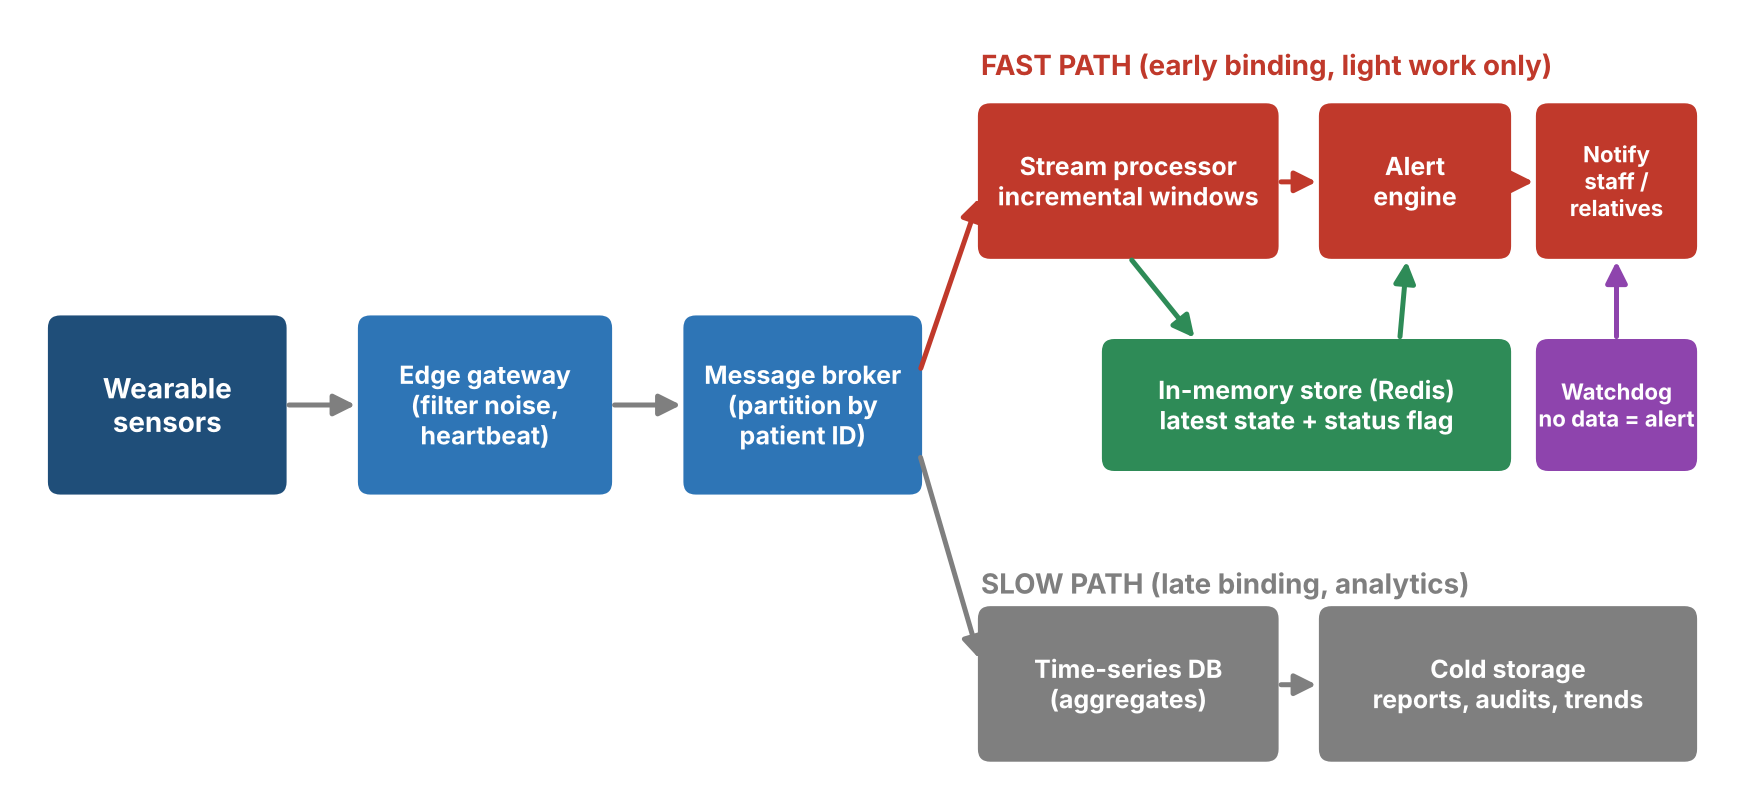
\includegraphics[width=\textwidth]{figures/fig_pipeline.png}
  \caption{Proposed data flow. The fast path (red) uses early binding; the slow path (grey) keeps late binding for analytics.}\label{fig:pipeline}
\end{figure}

\paragraph{Monitoring the monitor.} A \emph{watchdog} receives a heartbeat with every reading and raises a \texttt{DEVICE\_OFFLINE} alert when none arrives within a timeout. Pipeline lag should also be tracked, so that a delay is itself an alert. Redundant brokers, several alert channels (SMS, call, app) and an escalation chain when nobody acknowledges complete the design.

\paragraph{Replay of the incident.} The Java program \texttt{FailureSimulation} generates one reading per second for three patients over 600\,s (Figure~\ref{fig:watchdog}). Patient~2 has a tachycardia episode, and the 5-second average (early binding) crosses 120\,bpm, raising a threshold alert at $t=\tachyTime$\,s. The device of patient~3 stops at $t=\failTime$\,s. No threshold rule can fire without data, but the watchdog (timeout 10\,s) raises \texttt{DEVICE\_OFFLINE} at $t=\offlineTime$\,s, \offlineDelay{} seconds after the last reading.

\begin{figure}[H]
  \centering
  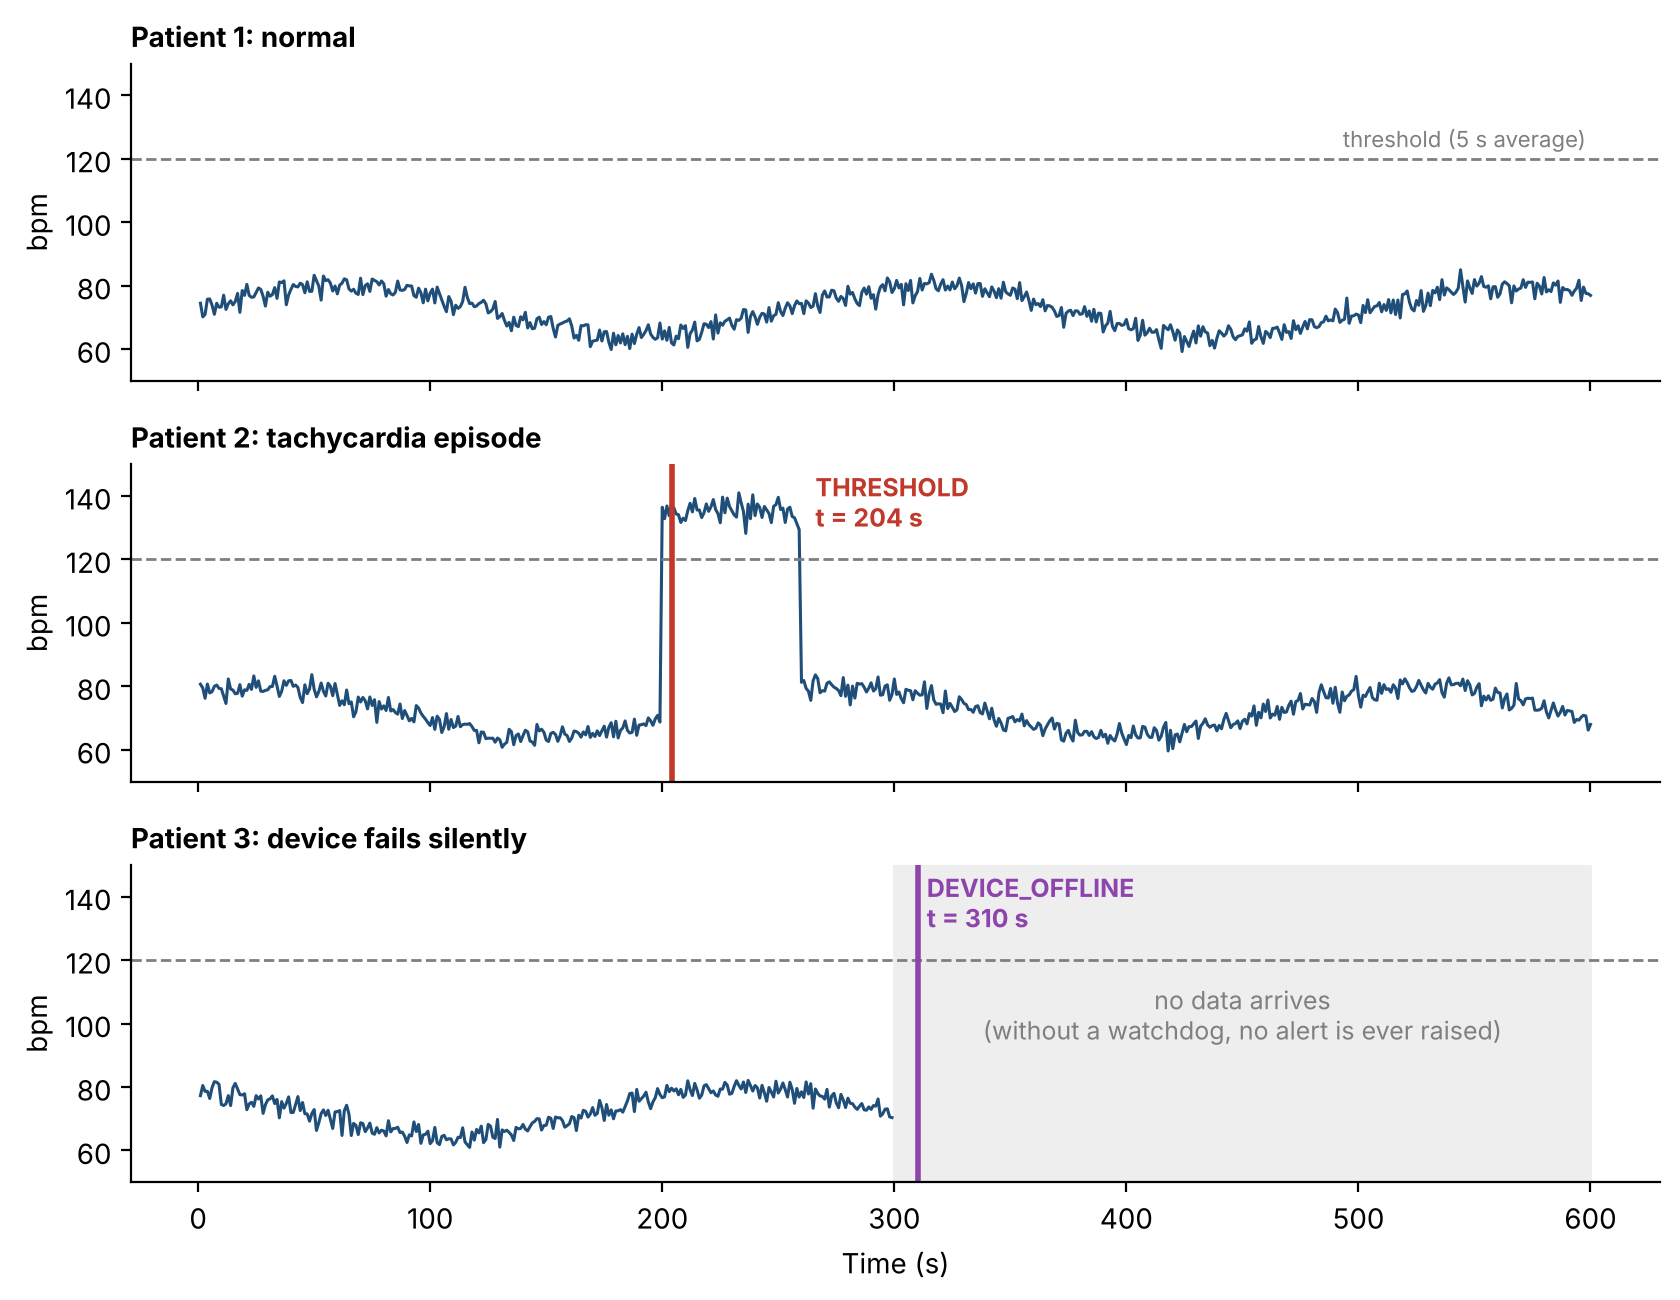
\includegraphics[width=0.95\textwidth]{figures/fig_watchdog.png}
  \caption{Simulated replay. Patient~2 triggers a threshold alert; the silent failure of patient~3 is caught only because of the watchdog.}\label{fig:watchdog}
\end{figure}

\section{Advantages and disadvantages of early binding}

\emph{Early binding} means performing computations earlier to avoid redundant work later~\cite{lecture}. In this context, indicators, aggregates and alert evaluations are computed and fixed at ingestion time, before anyone queries them. The trade-off is memory for time. The opposite idea, \emph{lazy evaluation}, delays computation until the value is required; it suits rarely used reports but not critical alerts, where waiting is dangerous.

\begin{table}[H]
\centering
\caption{Early binding in a real-time monitoring context.}\label{tab:prosandcons}
\begin{tabular}{@{}>{\raggedright\arraybackslash}p{7.4cm}>{\raggedright\arraybackslash}p{7.4cm}@{}}
\toprule
\textbf{Advantages} & \textbf{Disadvantages}\\
\midrule
Alerts are fast and predictable: the indicator is already computed when needed. &
Uses more memory and storage for derived values.\\[3pt]
Eliminates repeated work, so it scales as data volume grows. &
Less flexible: a new indicator or changed formula means recomputing, and past data may need reprocessing.\\[3pt]
Many consumers (alerts, dashboard, reports) reuse the same precomputed value. &
Costs work on every reading, even if nobody queries the result.\\[3pt]
The system stays responsive when it matters most: emergencies. &
Stale values are a risk: a cached value that is not updated correctly could hide a real emergency.\\[3pt]
 & More complex design (rule versioning, late and out-of-order data).\\
\bottomrule
\end{tabular}
\end{table}

\paragraph{Experiment.} To quantify the benefit, the Java program compares two implementations that return the same 5-minute average heart rate (a sanity check verifies they agree before timing). \texttt{LateBindingAverage} stores all readings and rescans the history on each request. \texttt{EarlyBindingAverage} keeps a running sum in a circular buffer of primitive arrays and updates it as each reading arrives. Each value is the median of nine timed trials after a discarded warm-up (Java \javaVersion, \cpuCores{} CPU cores; absolute values depend on the machine).

\begin{figure}[H]
  \centering
  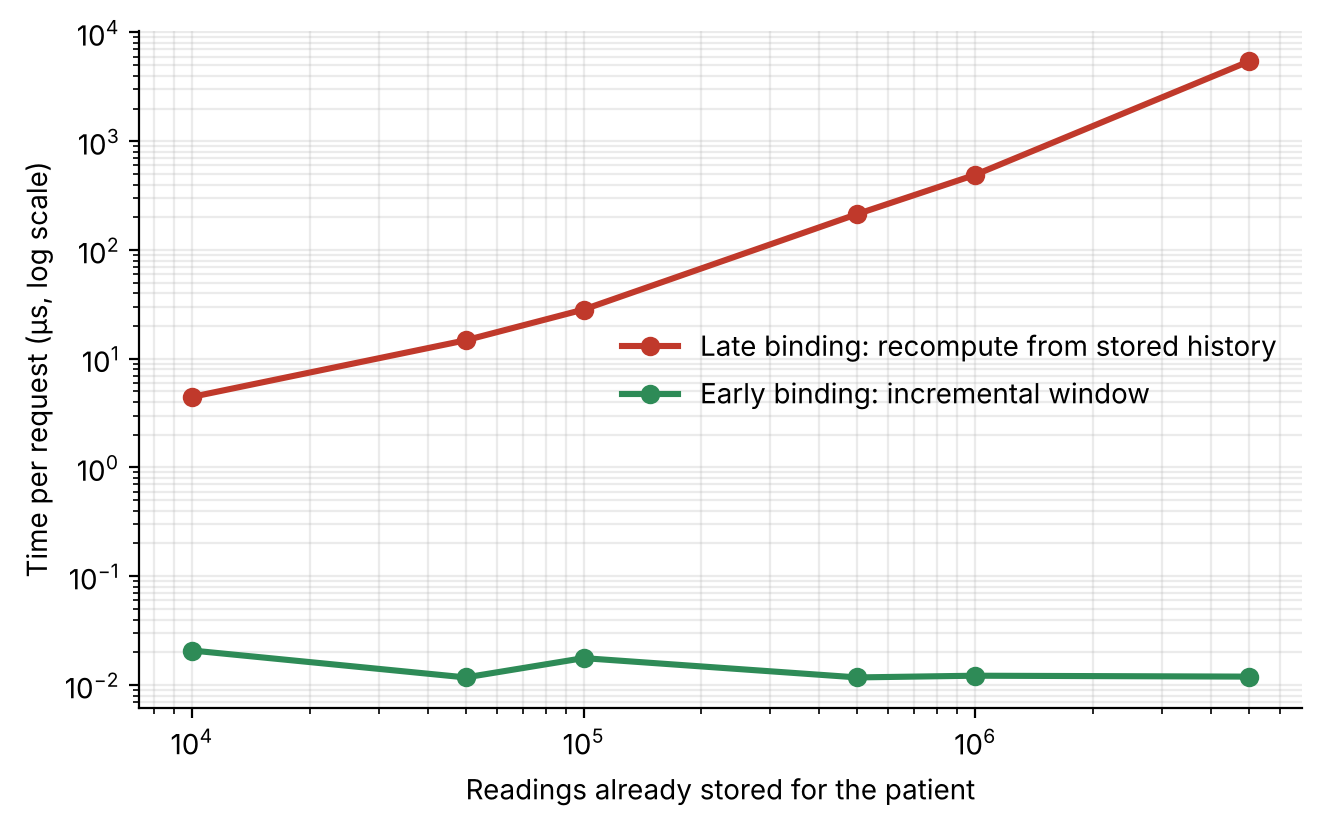
\includegraphics[width=0.85\textwidth]{figures/fig_benchmark.png}
  \caption{Measured time per request (log--log). The late-binding cost grows linearly with the stored history; the early-binding cost is flat.}\label{fig:benchmark}
\end{figure}

\begin{table}[H]
\centering
\caption{Measured results.}\label{tab:benchmark}
{\small\setlength{\tabcolsep}{4pt}\begin{tabular}{rrrrr}
\toprule
Stored readings & Late binding (\textmu s) & Early binding (ns) & Speed-up ($\times$) & Cores needed (late)$^{*}$ \\
\midrule
10\,000 & 4.5 & 20.8 & 210 & 0.004 \\
50\,000 & 14.8 & 11.7 & 1\,300 & 0.015 \\
100\,000 & 28.3 & 17.7 & 1\,600 & 0.028 \\
500\,000 & 214.0 & 11.7 & 18\,000 & 0.214 \\
1\,000\,000 & 491.2 & 12.2 & 40\,000 & 0.491 \\
5\,000\,000 & 5\,419.8 & 11.9 & 450\,000 & 5.420 \\
\bottomrule
\end{tabular}
}\\[3pt]
{\footnotesize $^{*}$ Derived, not measured: assumes 1\,000 patients sending one reading per second, one recomputation per reading, on one thread.}
\end{table}

\paragraph{Reading the results.} For a single patient the absolute cost of late binding is small at moderate history sizes: Java with primitive arrays scans millions of values in milliseconds. The problem is how the cost scales. It grows linearly with the history and is paid on every request, for every patient and every metric. With the assumptions of Table~\ref{tab:benchmark}, recomputation needs more than one full CPU core once the history reaches a few million readings (about 58 days of 1\,Hz data), whereas the incremental update stays negligible. This is the mechanism behind the delays reported in the case. The experiment is deliberately simple (one metric, synthetic data, a single thread) and shows the trend, not the performance of a production system.

\paragraph{Conclusion.} Use early binding for a small set of critical, well-defined indicators (heart rate, SpO$_2$, blood pressure, trends). Keep late binding or lazy evaluation for exploratory and historical analysis. A hybrid approach is best.

\paragraph{Optimization ethics.} Knuth warns that premature optimization is the root of all evil~\cite{knuth1974}, and Jackson's first rule of optimization is ``Don't do it''~\cite{jackson1975}. Here the optimization is justified because the failure revealed a real problem: delays under load. Even so, the best practices of the course still apply: profile first to confirm that recomputation is the bottleneck, keep the alert logic correct and clear before making it fast, and measure the improvement afterwards (which is what the benchmark does).

\section{How can pre-computed values be stored for fast retrieval?}

Storing precomputed values is memoization and caching applied to the platform. Different layers serve different purposes (Table~\ref{tab:storage}).

\begin{table}[H]
\centering
\caption{Storage layers for precomputed and raw data.}\label{tab:storage}
\begin{tabular}{@{}>{\raggedright\arraybackslash}p{6.2cm}>{\raggedright\arraybackslash}p{8.6cm}@{}}
\toprule
\textbf{Layer} & \textbf{Purpose}\\
\midrule
In-memory key-value store (e.g.\ Redis) & Latest state per patient with instant lookup.\\
Stream-processor state & Sliding windows and running aggregates kept next to the computation.\\
Time-series database with continuous aggregates & Per-minute or hourly summaries for dashboards and trends.\\
Cold storage (data lake or warehouse) & Raw data kept only for audits and analysis.\\
\bottomrule
\end{tabular}
\end{table}

\paragraph{Example record.}
\begin{lstlisting}[language={},numbers=none]
key:   patient:1042:vitals:latest
value: { heart_rate: 118, spo2: 91,
         hr_avg_5min: 104, trend: "rising",
         status: "WARNING", rule_version: 3,
         last_update: "2026-11-02T19:20:05Z" }
\end{lstlisting}

\paragraph{Design points.}
\begin{itemize}
  \item \textbf{Key by patient, metric and window}, so retrieval is a direct lookup and not a scan (data-structure optimization, memory layout and locality).
  \item \textbf{Store the alert status as a flag}, so the notifier reads a single value.
  \item \textbf{Keep a timestamp on each value.} If it is too old, treat it as a possible device failure; this also removes the stale-cache risk.
  \item \textbf{Version the rules.} Thresholds differ per patient (e.g.\ chronic conditions), so store which rule version produced each value.
  \item \textbf{Plan for failure:} use replication and snapshots, and be able to rebuild derived values from the raw stream.
\end{itemize}

\section{Implementation}

The repository contains the Java program (package \texttt{monitoring}) and the Python script that produces all figures and tables from its output. The early-binding structure and the watchdog are shown in Listings~\ref{lst:early} and~\ref{lst:watchdog}; the remaining classes (\texttt{LateBindingAverage}, \texttt{Benchmark}, \texttt{FailureSimulation}, \texttt{Main}) are in the repository. The early-binding class applies three rules of the course: it stores the running sum (\emph{don't do it again}), touches each reading once on entry and once on exit (\emph{do it less}), and uses primitive arrays in a circular buffer (\emph{primitives versus objects}, memory locality).

\lstinputlisting[caption={Incremental sliding-window average (early binding).},label={lst:early}]{listings/EarlyBindingAverage.java}

\lstinputlisting[caption={Watchdog that detects silent devices.},label={lst:watchdog}]{listings/Watchdog.java}

\noindent Repository: \url{https://github.com/YOUR-USER/YOUR-REPO}

\section{Conclusion}

The incident shows that recalculating every value on demand does not scale in a real-time medical system. Applying Bentley's rules, specifically \emph{Do it, but don't do it again} (caching) and \emph{Early binding}, critical indicators should be computed incrementally at ingestion and stored in a fast in-memory or time-series layer, separate from the analytical path. The experiment shows the cost of recomputation growing with history while the incremental update stays constant, and the replay shows that a watchdog closes the monitoring gap for silent devices. The costs are extra memory, less flexibility and the risk of stale data, which timestamps and rule versioning mitigate. Consistent with the optimization ethics of Knuth and Jackson, the changes should be justified by measurement and must keep the alert logic correct.

\bibliographystyle{plain}
\bibliography{references}

\end{document}
